\section{Desarrollo}
En esta sección describiremos los métodos usados para resolver el problema, cada uno con sus
ventajas y desventajas.

\subsection{Archivo de entrada}
\subsubsection{Explicacion}
El ejecutable toma tres parámetros por línea de comando, que serán el \textit{path} del archivo de entrada, el \textit{path} del archivo de salida y la estrategia que utilizaremos con el arquero.

El archivo de entrada seguirá el siguiente formato:
\begin{itemize}
	\item La primera línea contendrá la posición inicial del arquero en y, luego las coordenadas que defininen los límietes del arco, también sobre el eye y. Se asume que la posición en x del arquero y de la línea de gol son las mismas: $x = 125$. Finalmente estará $\mu$, la cota sobre el máximo desplazamiento que puede realizar el arquero en un instante de tiempo.
	\item Luego se muestra la secuencia de posiciones en $\mathbb{R}^2$, una por lína, que toma la pelota para los instantes de tiempo $0, \ 1, \ldots, T$, siendo $T$ el tiempo final.
\end{itemize}

En un primer lugar, leeremos la primera línea del archivo de entrada para \textit{setear} los valores correctos de la posición en y del arquero, las posiciones de los palos y el $\mu$. Luego, dado que se asume que no podemos saber qué pasará más allá del tiempo actual, iremos leyendo la entrada a medida que hagamos hecho los cálculos para el tiempo anterior.

\subsection{Archivo de salida}
\subsubsection{Explicacion}
El archivo de salida especificado como parámetro será creado en caso de que no exista y reemplazado por uno nuevo en caso de que ya exista. Este nuevo archivo contendrá una instrucción por línea, correspondiente a la acción que realiza el arquero en el instante $0 \leq t \leq T$, siendo $T$ el instante final.

Este archivo luego podrá ser usado junto con el archivo de entrada para analizar qué sucede con el visualizador proporcionado por la cátedra.

%%%%%%%%%%%%%%%%%%%%%%%%%%%%%%%%%%%%%%%%

\subsection{Método Uno: Usando Cuadrados Mínimos}
\subsection{Método Uno: Usando Cuadrados Mínimos}
Nuestro primer enfoque fue mirar al problema como si fuera uno de analizar los datos obtenidos en un
experimento y tratásemos de describir la distribución de estos mediante una función.

En esta perspectiva, nuestra entrada sería el tiempo y la salida la posición en la cancha de la
pelota. Además, como las variaciones en las coordenadas $x$ e $y$ de la pelota son independientes
podemos dividir al problema en una entrada y dos salidas. De esta forma, deberíamos resolver dos
problemas de cuadrados mínimos.

\subsubsection{Cuadrados Mínimos: General con Funciones Normales}
La siguiente información sobre \texttt{Cuadrados Mínimos} fue sacada de \cite[p~501]{burden}:

El problema general de aproximar un conjunto de datos, $\{(x_i, y_i) | i = 1,2, \ldots, m\}$ con un
polinomio
\begin{center}
  $P_n = a_n x^n + a_{n-1}x^{n-1}+ \hdots + a_1x+a_0,   $
\end{center}
de grado $n < m-1$, se reduce a elegir las constantes $a_0, a_1, \ldots, a_n$ que minimicen el
cuadrado mínimo $E = E_2(a_0, a_1,\ldots, a_n) donde$
\begin{center}
  $E = \sum_{i=1}^{m} (y_i - Pn(x_i))^2$

  $= \ldots  $\footnote{Para el desarrollo completo referirse al libro citado} $=$

  $ = \sum_{i=1}^{m} y_i^2 -2 \sum_{j=0}^{n} a_j \left(\sum_{i=1}^{m} y_i x_i^j \right) + 
    \sum_{j=0}^{n} \sum_{k=0}^{n} a_j a_k \left(x_i^{j+k}\right)$
\end{center}

Para encontrar los mínimos, dado que es una función convexa (falta demostrar), debemos buscar los
puntos críticos y éstos serán los mínimos globales. Para ello, diferenciaremos la función por sus
constantes $a_i$ y las igualaremos a 0:
\begin{center}
  $0 =  \frac{\partial E}{\partial a_j}$
\end{center}
Lo que daría, después de algunos pasos$^1$, $n+1$ ecuaciones del siguiente estilo, con $0 \leq k
\leq n$:
\begin{center}
  $a_o \sum{i=1}{m} x_i^{k} + a_1 \sum{i=1}{m} x_i^{k+1}+ a_2 \sum{i=1}{m} x_i^{k+2} + \hdots +
   a_n \sum{i=1}{m} x_i^{k+n} =   \sum{i=1}{m} y_i x_i^k$
\end{center}

Estas ecuaciones terminarían formando las filas de nuestra matriz extendida y el sistema
lineal\footnote{Es lineal dado que las incógnitas están relacionadas entre ellas de forma lineal}
resultante tiene solución única si los $x_i$ distintos.

\subsubsection{Cuadrados Mínimos: Nuestro trabajo}

Adaptado a nuestro trabajo, tendríamos dos sistemas lineales de ecuaciones de $n+1$ filas y $n+1$
columnas representando las funciones normales con entrada $t$ tiempo y salida coordenada $x$; y
entrada $t$ tiempo y salida coordenada $y$, respectivamente.

Es decir, para poder describir el comportamiento de ambas variables con un polinomio de grado como
máximo n, necesitaríamos n+1 tiempos.



\subsubsection{Resolver Cuadrados Mínimos usando QR}
Sea A = Q*R la factorización QR de la matriz A mencionada en las secciones anteriores. Entonces, 
\begin{center}
 $\displaystyle \min_{x \in \mathbb{R}^{(n+1)}} \| Ax-b\|^2 = \min_{x \in \mathbb{R}^{(n+1)}} \| Q^tAx-Q^tb \|^2 = \min_{x \in \mathbb{R}^{(n+1)}} \| Rx-Q^tb\|^2$
\end{center}
Como A tiene columnas independientes\footnote{Para más información, referirse a la sección demostraciones}, entonces $R_{i,i} \neq 0 \ \forall i=1,\ldots,n+1$ 
y además {$R_{i,j} = \nobreak 0 \ \forall i=1,\ldots,m; \ j=1,\ldots,i-1 $}. La multiplicacion matriz-vector Rx entonces sería:
\begin{center}
$Rx = \begin{pmatrix}
        R_1x \\
        0
       \end{pmatrix}$ con $R_1 \in \mathbb{R}^{(n+1) \times (n+1)}$ la parte por arriba de la diagonal de $R$.
\end{center}
Además, si reescribimos a $Q^tb$ como:
\begin{center}
$Q^tb = \begin{pmatrix}
        c\\
        d
       \end{pmatrix}$ con $c \in \mathbb{R}^{(n+1) \times (n+1)}$ y $d \in \mathbb{R}^{m-(n+1)}$, problema se reduce a:

$\min_{x \in \mathbb{R}^{(n+1)}} \| Rx-Q^tb\|^2 = \| (R_1x,0)^t -(c,d)^t \|^2 =
\min_{x \in \mathbb{R}^{(n+1)}} \|R_1x-c\|^2+\|d\|^2$

$ \rightarrow \min_{x \in \mathbb{R}^{(n+1)}} \| R_1x-c\|^2 \rightarrow x/ R_1x=c$
\end{center}

\begin{figure}[H] 
\begin{center}
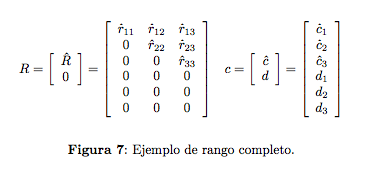
\includegraphics[width=0.6\textwidth]{img/exp-qr.png} 
\end{center}
\end{figure}


El sistema $R_1x=b$ tiene solución dado que $R_1$ es triangular superior con elementos no nulos en la diagonal. Si encontramos el $x$ que sea solución para ese sistema, será el mismo $x$ solución para el problema de Cuadrados Mínimos.





% %%%%%%%%%%%%%%%%%%%%%%%%%%%%%%

% Se plantea el nuevo sistema $Q^t A x = Q^t b$ que equivale a Rx = c, donde $\hat{c}$ son los primeros m elementos de c y d los restantes. El residuo s resulta s = c - Rx, donde los primeros m elementos de s son iguales a $\hat{c}$ - Rx y los restantes a d. De esta forma, el cuadrado del residuo, es decir, lo que se busca minimizar es igual a 

% \begin{center}
% $||$s$||^2_2$ = $||$ $\hat{c} - \hat{R}$x$||^2_2$ + $||$d$||^2_2$
% \end{center}

% Puesto que el segundo termino, d no depende de x, se busca minimizar el primero. Como $\hat{R}$ era no singular, entonces la solucion del sistema $\hat{R}$x = $\hat{c}$ es unica y es la solucion de cuadrados minimos. cabe destacar que el termino es la norma del residuo asociado con solucion obtenida.


\subsubsection{Pseudocodigo}

\begin{algorithm}[H]
\caption{FactorizacionQR(Matrix A $\in \mathbb{R}^{n \times m}$)}
\label{pseudo:Factorizacion-QR}
\begin{algorithmic}

\STATE Matriz $R \leftarrow A$

\STATE Matriz $Q \leftarrow$ Matriz Identidad $\in \mathbb{R}^{n \times n}$
\STATE Matriz $Qt \leftarrow$ Matriz Identidad $\in \mathbb{R}^{n \times n}$

\FOR{$i=0$ hasta $m$}
    \IF{$(n - i) > 1 $}
    %\COMMENT{tmp siempre tiene el mismo tamaño, a diferencia de subR y subQt}
    \STATE Matrix $tmp \leftarrow$ Matriz Identidad $\in \mathbb{R}^{n \times n}$
    \STATE Matrix $subQt \leftarrow$ Matriz Identidad $\in \mathbb{R}^{(n-i) \times (n-i)}$
    \STATE Matrix $subR \leftarrow generarSubMatriz(R,i) \in \mathbb{R}^{(n-i) \times (m-i)}$
     %  \COMMENT{Si no entra a acá, es el último caso y no es necesario triangular}
    \STATE $(subR, subQt) \leftarrow$ triangularColumna($subR, subQt)$
    \STATE $R \leftarrow$ agregarSubMatrix($subR, R, i)$
    \STATE $tmp \leftarrow$ agregarSubMatrix($subQt, tmp, i)	$
    \ENDIF
	\STATE $Qt \leftarrow tmp*Qt$
\ENDFOR
\STATE \textbf{return} $(Qt, R)$
\end{algorithmic}
\end{algorithm}


\begin{algorithm}[H]
\caption{generarSubMatrix(Matrix $A \in \mathbb{R}^{n \times m}$, int $i$)}
\label{pseudo:generar-sub-matrix}
\begin{algorithmic}
\STATE Matriz $res \leftarrow$ Matriz $\in \mathbb{R}^{(n-i) \times (m-i)}$
\STATE $res_{k,l} \leftarrow A_{i+k,i+l} \ \ \forall k=0,\ldots,(n-i)$ y $l=0,\ldots,(m-i)$
\STATE \textbf{return} $res$
\end{algorithmic}
\end{algorithm}



\begin{algorithm}[H]
\caption{triangularColumna(Matrix $sub \in \mathbb{R}^{n \times m}$, Matrix $subQt \in \mathbb{R}^{n \times m}$)}
\label{pseudo:triangular-columna}
\begin{algorithmic}

\STATE Vector x $\leftarrow$ Vector de Ceros$ \in \mathbb{R}^n$
\STATE Vector y $\leftarrow$ Vector de Ceros$ \in \mathbb{R}^n$
\STATE Vector u $\leftarrow$ Vector de Ceros$ \in \mathbb{R}^n$


\FOR{$i = 0$ hasta $x.n$}
  	\STATE $x_i \leftarrow sub_i$
\ENDFOR

\STATE $y_0 \leftarrow \| x \|$
\STATE $u \leftarrow x - y$

\STATE Vector $uTranspuesto \leftarrow u^t \in \mathbb{R}^{1 \times n}$
\STATE Vector $aux \leftarrow$ Vector $uTranspuesto*sub \ \in \mathbb{R}^n$
\STATE Matriz $aux2 \leftarrow$ Matriz $u*aux \ \in \mathbb{R}^{n \times m}$
\STATE int $coeficiente \leftarrow 2/\| u \| ^2$

\STATE $sub \leftarrow sub - (aux2*coeficiente)$

\STATE $aux \leftarrow uTranspuesto * subQt$
\STATE $aux2 \leftarrow u*aux$
\STATE $subQt \leftarrow subQt - (aux2 * coeficiente)$
\STATE \textbf{return} (sub, subQt)

\end{algorithmic}
\end{algorithm}


\begin{algorithm}[H]
\caption{agregarSubMatrix(Matrix $sub \in \mathbb{R}^{(n-i)\times (m-i)}$, Matrix $A \in \mathbb{R}^{n \times m}$, int $i$)}
\label{pseudo:agregar-sub-matrix}
\begin{algorithmic}
\STATE $A_{i+k,i+l} \leftarrow sub_{k,l} \ \ \forall k=0,\ldots,(n-i)$ y $l=0,\ldots,(m-i)$
\STATE \textbf{return} Matriz A modificada
\end{algorithmic}
\end{algorithm}

\input{texto/arquero.tex}

%%%%%%%%%%%%%%%%%%%%
El método de la potencia asume que tenemos un autovalor dominante y que todos los autovalores son
mayores o iguales a 0. $A^t A$ es simétrica por lo que tenemos una base ortonormal de autovectores
y además es semi-defininda positiva, por lo que sus autovalores son positivos o 0. El problema es
que no podemos asegurar que después de aplicar deflación, la matriz seguirá siendo semi-definida
positiva, aunque sí simétrica. En esta sección, demostraremos los supuestos que asumimos para
aplicar las técnicas en el trabajo.



\ \\

Sean $A \in \mathbb{R}^{n \times m}$, $A^t A \in \mathbb{R}^{m \times m}$, $\lambda \in \mathbb{R}$
, $v \in \mathbb{R}^m$ y $B = A^t A - \lambda_{1} v v^t$.

\ \\
\textbf{Lema:} la matriz $A^t A$ y $A A^t$ son simétricas.

\ \\
Prueba:

\begin{center}
  $(A^t A)^t = (A)^t (A^t)^t = A^t A$
  $(A A^t)^t = (A^t)^t (A)^t = A A^t$
\end{center}

(1) $A^t A$ simétrica y $v$ vector.
\ \\

\ \\
\textbf{Lema:} la matriz $B$ es simétrica

\ \\
Prueba:

\begin{center}
  $B_{ij} = (A^t A)_{ij} - \lambda v_i (v^t)_j = (A^t A)_{ij} - \lambda v_i v_j =^{(1)} (A^t A)_{ji}
  - \lambda v_j (v^t)_i = B_{ji}$
\end{center}

(1) $A^t A$ simétrica y $v$ vector.
\ \\


\ \\
\textbf{Lema:} Los valores singulares de $A$ son los mismos que los valores singulares de $A^t$.

\ \\
Prueba: Los valores singulares de la matriz $\Sigma$ son las raices de los autovalores en orden
decreciente por la diagonal. Los autovalores están definidos como los valores que anulan a la
función
$\psi(\lambda) = det(\lambda I - A)$. En el caso de la traspuesta, sus autovalores son los que
anulan a la función $\psi(\lambda) = det(\lambda I - A^t)$, pero $(\lambda I - A)^t = (\lambda I -
A^t)$ y el determinante es invariante al trasponer una matriz. Entonces los autovalores son los
mismos y, por ende, los valores singulares también.


\ \\
\textbf{Lema:} Si $A \in \mathbb{R}^{nxm},\Sigma \in \mathbb{R}^{mxn}, U \in \mathbb{C}^{mxm}, V \in
\mathbb{C}^{nxn}, A = U \Sigma V^t$, entonces:
\begin{compactitem}
  \item $A^t = V \Sigma U^t $ con $A^t \in \mathbb{R}^{m \times n}$
  \item $A A^t = U \Lambda U^t $ con $\Lambda$ la matriz con los autovalores de $A$ y $A^t$ en
    la diagonal y $A A^t \in \mathbb{R}^{n \times n}$.
  \item $A^t A = V \Lambda V^t $ con $\Lambda$ la matriz con los autovalores de $A$ y $A^t$ en
    la diagonal $A^t A \in \mathbb{R}^{m \times m}$.
\end{compactitem}

\ \\
Prueba: El primero es inmediato de trasponer $A$ y del hecho de que $\Sigma$ es diagonal. Para el
segundo y el tercero:
\begin{center}
$A A^t = U \Sigma V^t V \Sigma U^t =^{(1)} U \Sigma \Sigma U^t =^{(2)} U \Lambda U^t$

\ \\
$A^t A = V \Sigma U^t U \Sigma V^t =^{(1)} V \Sigma \Sigma V^t =^{(2)} V \Lambda V^t$
\end{center}

(1) $U$ y $V$ matrices ortogonales

(2) $\lambda$ diagonal con valores singulares en la diagonal.



